\documentclass[aspectratio=169, pdf, 8pt, unicode]{beamer}
\usepackage[american,russian]{babel}
\usepackage[default]{sourcesanspro}
\usepackage{float}
\usepackage{graphicx}
\usepackage{pgfplotstable}
\usepackage{caption}
\usepackage{amsmath}
\usepackage{amssymb}
\usepackage{setspace}
\usepackage{fancyvrb}
\usepackage[outputdir=aux]{minted}

\DeclareCaptionLabelFormat{gostfigure}{Рисунок #2}
\captionsetup[table]{labelsep=endash,justification=justified,singlelinecheck=false,font=normalsize,skip=0pt} 
\captionsetup[figure]{labelformat=gostfigure,labelsep=endash,justification=centering,singlelinecheck=false,font=normalsize} 
\pgfplotsset{compat=1.9}

\mode<presentation> {
\usetheme{Madrid}
}

\setbeamerfont{institute}{size=\normalsize}
\setbeamertemplate{itemize/enumerate body begin}{\large}
\setbeamertemplate{itemize/enumerate subbody begin}{\tiny}

\title[Теория и практика многопоточного программирования]{Теория и практика многопоточного программирования\\ \vspace{0.5cm}Семинар 3}

\author{Неганов Алексей}

\institute[МФТИ]{
    Московский физико-технический институт (национальный исследовательский университет)\\
    Кафедра теоретической и прикладной информатики\\
}

\date{Москва 2020}

\setbeamertemplate{caption}[numbered]

\begin{document}

\begin{frame}
\titlepage
\end{frame}

\begin{frame}[fragile]
\frametitle{Неатомарные операции}
\begin{itemize}
\item Инструкция процессора, работающая с невыровненным адресом
\begin{figure}[H]
\begin{BVerbatim}
struct  __attribute__((__packed__)) my_struct {
   char padding[2];
   int32_t cnt;
};
\end{BVerbatim}
\end{figure}
\item Инструкция процессора, работающая с выровненным адресом
\begin{figure}[H]
\begin{BVerbatim}
strd r0, r1, [r2] ; ARMv7
\end{BVerbatim}
\end{figure}
\item Любая операция языка C
\end{itemize}
\end{frame}


\begin{frame}
\frametitle{Атомарные регистры}
\begin{block}{Теорема}
   Если поведение соисполняемого регистра удовлетворяет условиям:
   \begin{enumerate}
      \item $\nexists i \: R^i \rightarrow W^i$ (ни одно чтение не может вернуть значение из будущего),
      \item $\nexists j \: W^i \rightarrow W^j \rightarrow R^i$ (ни одно чтение не может вернуть значение из отдалённого прошлого),
      \item если $R^i \rightarrow R^j$, то $i \leqslant j$,
   \end{enumerate}
   то такая реализация является атомарной.
\end{block}

\end{frame}

\begin{frame}[fragile]
\frametitle{Алгоритм <<булочной>> Лампорта}
\begin{figure}[H]
\centering
\begin{minipage}{0.8\textwidth}
\begin{minted}{C}
bool entering[n];
int num[n] = {0};

void lock(int i) {
   // choose number
   entering[i] = true;
   num[i] = max(num[0], ..., num[n-1]) + 1;
   entering[i] = false;

   for (j = 0; j < n; j++) {
      // wait until thread j receives its number
      while(entering[j]);

      // wait for threads with smaller numbers or same number and smaller index
      while(num[j] > 0 && (num[j] < num[i] || (num[j] == num[i] && j < i)));
   }
}

void unlock(int i) {
   num[i] = 0;
}
\end{minted}
\end{minipage}
\end{figure}
\end{frame}

\begin{frame}[fragile]
\frametitle{RMW-операции}
CAS:
\begin{figure}[H]
\centering
%\begin{BVerbatim}
\begin{minipage}{0.8\textwidth}
\begin{minted}{C}
bool bool_compare_and_swap(type *ptr, type oldval, type newval) {
   if (*ptr == oldval) {
      *ptr = newval;
      return true;
   }
   else
      return false;
}

type val_compare_and_swap(type *ptr, type oldval, type newval) {
   if (*ptr == oldval) {
      *ptr = newval;
      return newval;
   }
   else
      return *ptr;
}
\end{minted}
\end{minipage}
%\end{BVerbatim}
\end{figure}
\end{frame}

\begin{frame}[fragile]
\frametitle{RMW-операции}
Реализация прочих примитивов:
\begin{figure}[H]
\centering
%\begin{BVerbatim}
\begin{minipage}{0.8\textwidth}
\begin{minted}{C}
type fetch_and_add(type *ptr, type value) {
   int cur;
   do {
      cur = *ptr;
   } while (!bool_compare_and_swap(ptr, cur, cur + value));
   return cur;
}
\end{minted}
\end{minipage}
%\end{BVerbatim}
\end{figure}
Типичный паттерн использования:
\begin{figure}[H]
\centering
%\begin{BVerbatim}
\begin{minipage}{0.8\textwidth}
\begin{minted}{C}
while (1) {
   oldval = *ptr;
   newval = /* ... */
   if (bool_compare_and_swap( ptr, oldval, newval))
      break;
}
\end{minted}
\end{minipage}
%\end{BVerbatim}
\end{figure}
\end{frame}

\begin{frame}[fragile]
\frametitle{RMW-операции: ABA}

\begin{minipage}{0.4\textwidth}
\begin{small}
\begin{verbatim}
 1 struct node {
 2       struct node *next;
 3 }
 4
 5 static struct node *top = NULL;
 6 
 7 void push(struct node *n) {
 8       do {
 9             struct node *t = top;
10             n->next = t;
11       while (!CAS(&top, t, n));
12 }
13
14 void struct node *pop(void) {
15       struct node *next;
16       do {
17             struct node *t = top;
18             if (t == NULL)
19                   return NULL;
20             next = t->next;
21       } while (!CAS(&top,t,next));
22       return t;
23 }
\end{verbatim}
\end{small}
\end{minipage}%
\begin{minipage}{0.4\textwidth}
Пусть имеются два потока, выполняющий каждый следующие действия:

\begin{small}
\begin{verbatim}
Поток #1:                      Поток #2:

struct node *a = pop();        struct node *b = pop();
                               pop();
                               push(b);
\end{verbatim}
\end{small}

Может ли этот код привести к некорректному состоянию стека? Если да, на каких строках должно произойти переключение контекста?
\end{minipage}%
\end{frame}

\begin{frame}[fragile]
\frametitle{RMW-операции: ABA}
LL/SC:
\begin{figure}[H]
\centering
%\begin{BVerbatim}
\begin{minipage}{0.8\textwidth}
\begin{minted}{C}
word LL(word *ptr) {
   return *ptr; // and set cache line status bit simultaneously
}

bool SC(word *ptr, word newval) {
   if ( /* cache line bit is set */ ) {
      *ptr = newval;
      return true ;
   }
   else
      return false ;
}

bool CAS(word *ptr, word oldval, word newval) {
   if (LL(ptr) == oldval)
      return SC(ptr, newval);
   return false ;
}
\end{minted}
\end{minipage}
%\end{BVerbatim}
\end{figure}
\end{frame}

\begin{frame}[fragile]
\frametitle{Барьеры памяти}
\hspace{0.05\textwidth}
\begin{minipage}{0.2\textwidth}
\begin{figure}[H]
\centering
\begin{BVerbatim}
int a = 0;
int b = 0;

void foo(void) {
      a = 1;
      b = 1;
}

void bar(void) {
      while(b == 0);
      assert(a == 1);
}
\end{BVerbatim}
\end{figure}
\end{minipage}
\begin{minipage}{0.7\textwidth}
\begin{figure}[H]
      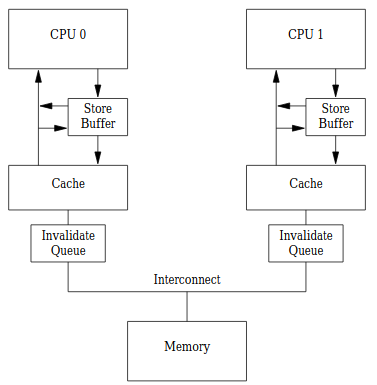
\includegraphics[width=0.5\textwidth]{fig/store_buffers.png}
\end{figure}
\end{minipage}
\end{frame}

\begin{frame}[fragile]
\frametitle{Барьеры памяти}
\hspace{0.05\textwidth}
\begin{minipage}{0.2\textwidth}
\begin{figure}[H]
\centering
\begin{BVerbatim}
int a = 0;
int b = 0;

void foo(void) {
      a = 1;
      smp_wmb();
      b = 1;
}

void bar(void) {
      while(b == 0);
      smp_rmb();
      assert(a == 1);
}
\end{BVerbatim}
\end{figure}
\end{minipage}
\begin{minipage}{0.7\textwidth}
\begin{figure}[H]
      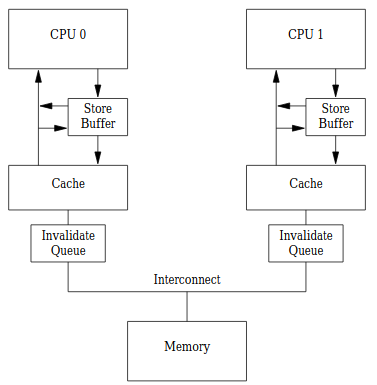
\includegraphics[width=0.5\textwidth]{fig/store_buffers.png}
\end{figure}
\end{minipage}
\end{frame}

\begin{frame}[fragile]
\frametitle{Модели памяти: sequentially consistent}
\begin{figure}[H]
\begin{BVerbatim}
atomic_t x, y;
x.store(0);
y.store(0);

y.store(20);      if (x.load() == 10) {          if (y.load() == 10)
x.store(10);        assert (y.load() == 20)        assert (x.load() == 10);
                    y.store (10);
                  }
\end{BVerbatim}
\end{figure}
Load/store операции могут выполняться лишь в том порядке, что и в коде, ни один \texttt{assert} выполниться не может.
\begin{figure}[H]
\begin{BVerbatim}
atomic_t x;
x.load(0);
int y = 0;

y = 1            if (x.load() == 2)
x.store(2);        assert (y == 1)
\end{BVerbatim}
\end{figure}
Запись в $y$ в коде происходит до записи в $x$, следовательно, \texttt{assert} выполниться не может.
\end{frame}

\begin{frame}[fragile]
\frametitle{Модели памяти: relaxed}
\begin{figure}[H]
\begin{BVerbatim}
// 'memory_order_relaxed' argument is omitted for brevity
atomic_t x, y;
x.store(0);
y.store(0);

y.store(20);      if (x.load() == 10) {          if (y.load() == 10)
x.store(10);        assert (y.load() == 20)        assert (x.load() == 10);
                    y.store (10);
                  }
\end{BVerbatim}
\end{figure}
Load/store операции могут переупорядочиваться, может сработать и тот, и другой \texttt{assert}.
\begin{figure}[H]
\begin{BVerbatim}
x.store(1);      y = x.load();
y.store(2);      z = x.load();
                 assert(y <= z);
\end{BVerbatim}
\end{figure}
Гарантия -- \texttt{assert} не может сработать.
\end{frame}

\begin{frame}[fragile]
\frametitle{Модели памяти: acquire/release}
\begin{figure}[H]
\begin{BVerbatim}
load memory, register ;
membar #LoadLoad | #LoadStore ; // acquire barrier

...

membar #LoadStore | #StoreStore ; // release barrier
store regiser, memory
\end{BVerbatim}
\end{figure}
\end{frame}

\begin{frame}[fragile]
\frametitle{Модели памяти: acquire/release}
\begin{figure}[H]
\begin{BVerbatim}
#define A memory_order_acquire
#define R memory_order_release

// thread 1                                   // thread 2
y.store(20, R);                               x.store(10, R);

// thread 3                                   // thread 4
assert(y.load(A) == 20 && x.load(A) == 0);    assert(y.load(A) == 0 && x.load(A) == 10); 
\end{BVerbatim}
\end{figure}

В sequential consistency один из \texttt{assert} сработает, в acquire/release --- оба могут пройти.

\begin{figure}[H]
\begin{BVerbatim}
// 'memory_order_XXX' argument is omitted for brevity
atomic_t x, y;
x.store(0);
y.store(0);

y.store(20);      if (x.load() == 10) {          if (y.load() == 10)
x.store(10);        assert (y.load() == 20)        assert (x.load() == 10);
                    y.store (10);
                  }
\end{BVerbatim}
\end{figure}

В acquire/release \texttt{assert} второго потока пройдёт, а третьего --- сработает.

\end{frame}

\begin{frame}[fragile]
\frametitle{Spinlock}
\begin{figure}[H]
\centering
\begin{minipage}{0.8\textwidth}
\begin{minted}{C++}
class spin_lock 
{
    atomic<unsigned int> m_spin ;
public:
    spin_lock(): m_spin(0) {}
    ~spin_lock() { assert( m_spin.load(memory_order_relaxed) == 0);}

    void lock()
    {
        unsigned int nCur;
        do { nCur = 0; }
        while ( !m_spin.compare_exchange_weak( nCur, 1, memory_order_acquire ));
    }
    void unlock()
    {
        m_spin.store( 0, memory_order_release );
    }
};
\end{minted}
\end{minipage}
\end{figure}
\end{frame}

\begin{frame}
\frametitle{Задачи}
\begin{enumerate}
\item Напишите свой mutex, использующий exponential backoff. Придумайте тесты для сравнения обычного spinlock и вашей реализации.
   Желательно использовать C++11 (и выше), при желании можно GNU С.
\item Напишите реализацию односвязного списка, поддерживающего чтение и вставку \textbf{(пока без удаления)}, безопасного в многопоточной среде,
   используя примитив CAS. Сравните реализации на C++11 и GNU C.
\end{enumerate}

Доклады:
\begin{enumerate}
\item Протоколы MESI, MOESI, MESIF.
\item Барьеры памяти в x86 с примерами на ассемблере. Связь с memory order из C11 / C++11.
\end{enumerate}

\end{frame}

\end{document}
